\section{Results}

\begin{figure}[!htbp]
  \begin{center}
%  {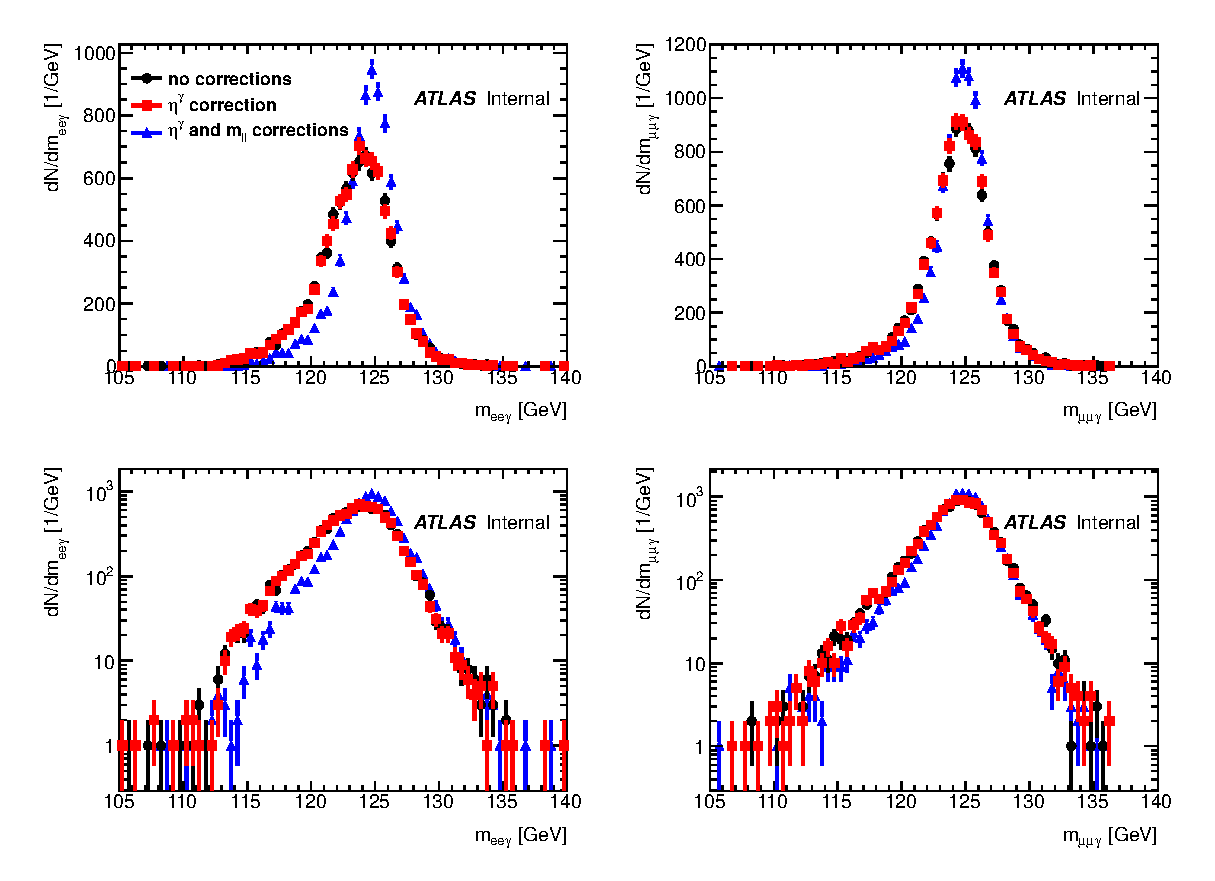
\includegraphics[width=0.99\textwidth]{figures/signal_mllg_corrections}}
{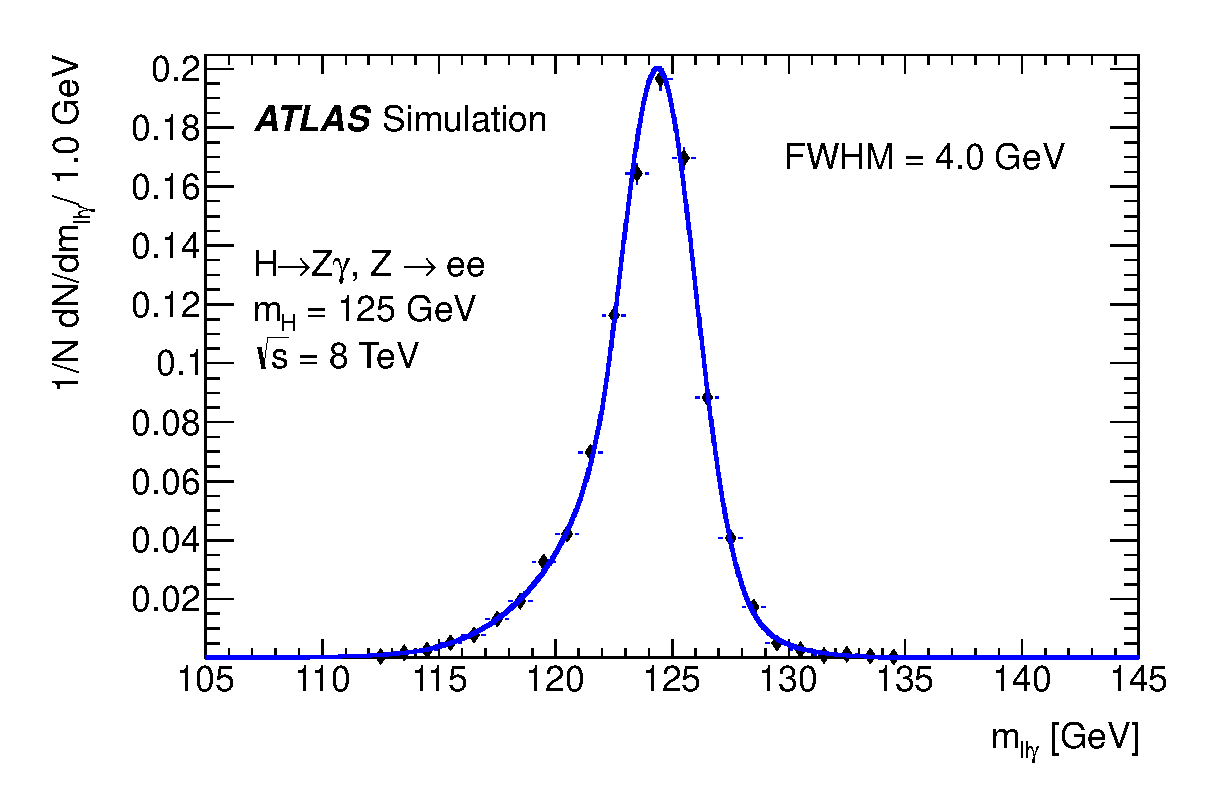
\includegraphics[width=0.48\textwidth]{figures/PlotsSuperposedResolutionCorrections_e_mc12a_Mllg}}
{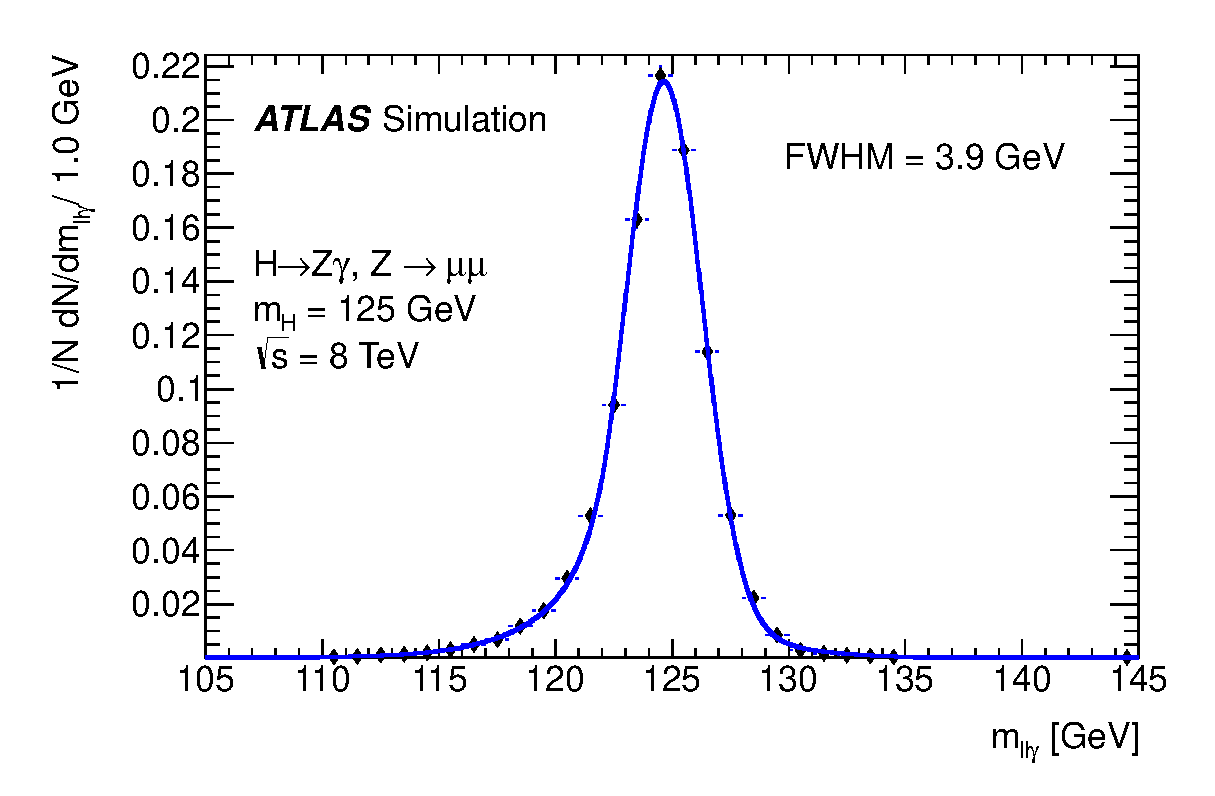
\includegraphics[width=0.48\textwidth]{figures/PlotsSuperposedResolutionCorrections_mu_mc12a_Mllg}}
\caption{Three-body invariant mass distribution for $gg\to H\to Z\gamma$
    selected events in the 8 TeV, $m_H=125$~GeV signal simulation, 
    after applying all analysis cuts and corrections. The blue solid lines 
    represent the fits to the points of the sum of a 
    Crystal Ball lineshape and a Gaussian function.
    Left: $Z\to ee$ channel, right: $Z\to\mu\mu$ channel.}
%the standard reconstruction (red circles), and after choosing the event primary vertex as the photon origin and applying the $Z$ mass constraint to the lepton four momenta (blue diamonds). The (dashed) red line and the (blue) solid line  represent the fits to the points of the sum of a Crystal Ball lineshape and a Gaussian function. Left: $Z\to ee$ channel, right: $Z\to\mu\mu$ channel.}
  \label{fig:signal_resolution_corrections}
  \end{center}
\end{figure}

\begin{figure}[!htbp]
  \begin{center}
    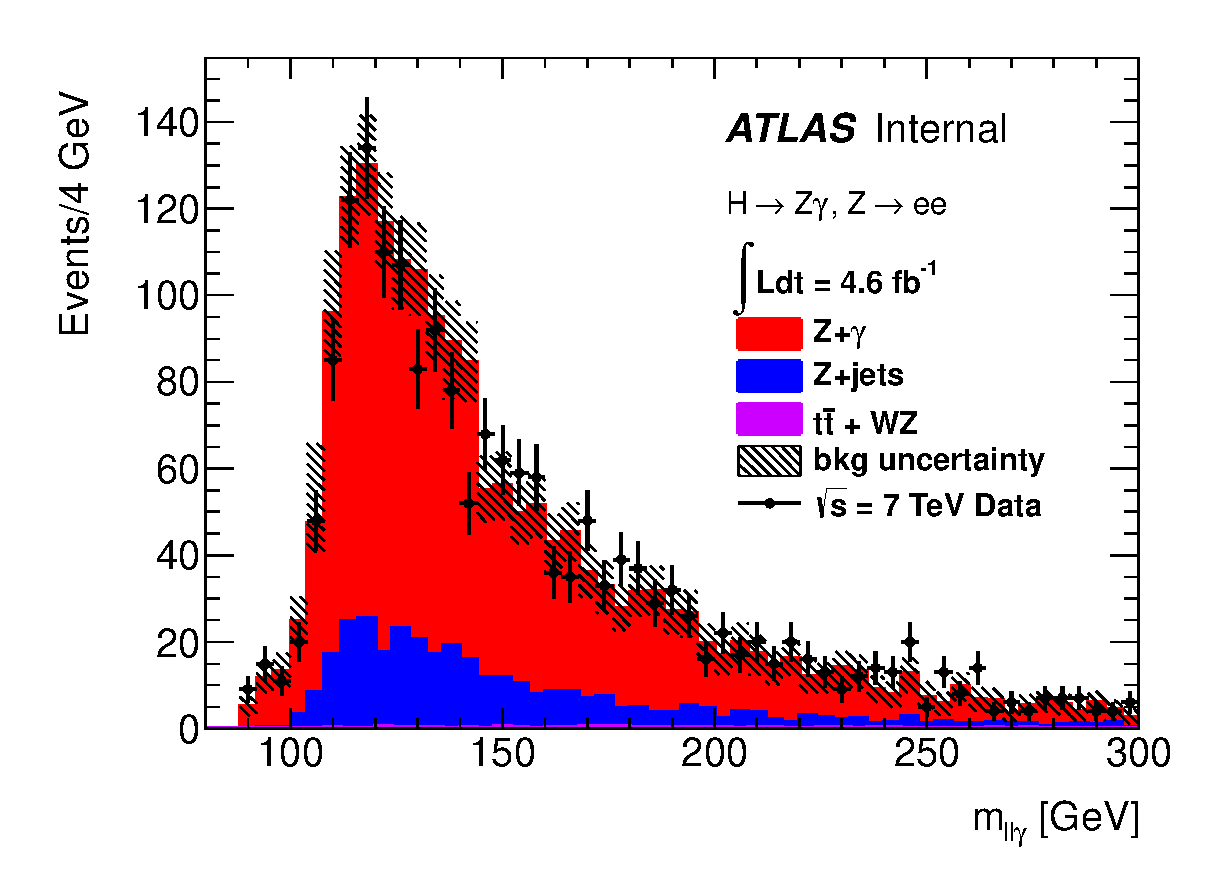
\includegraphics[width=0.49\columnwidth]{figures/bkg_decomposition_2011_e_Mllg_Z_PV_corr_linscale}
    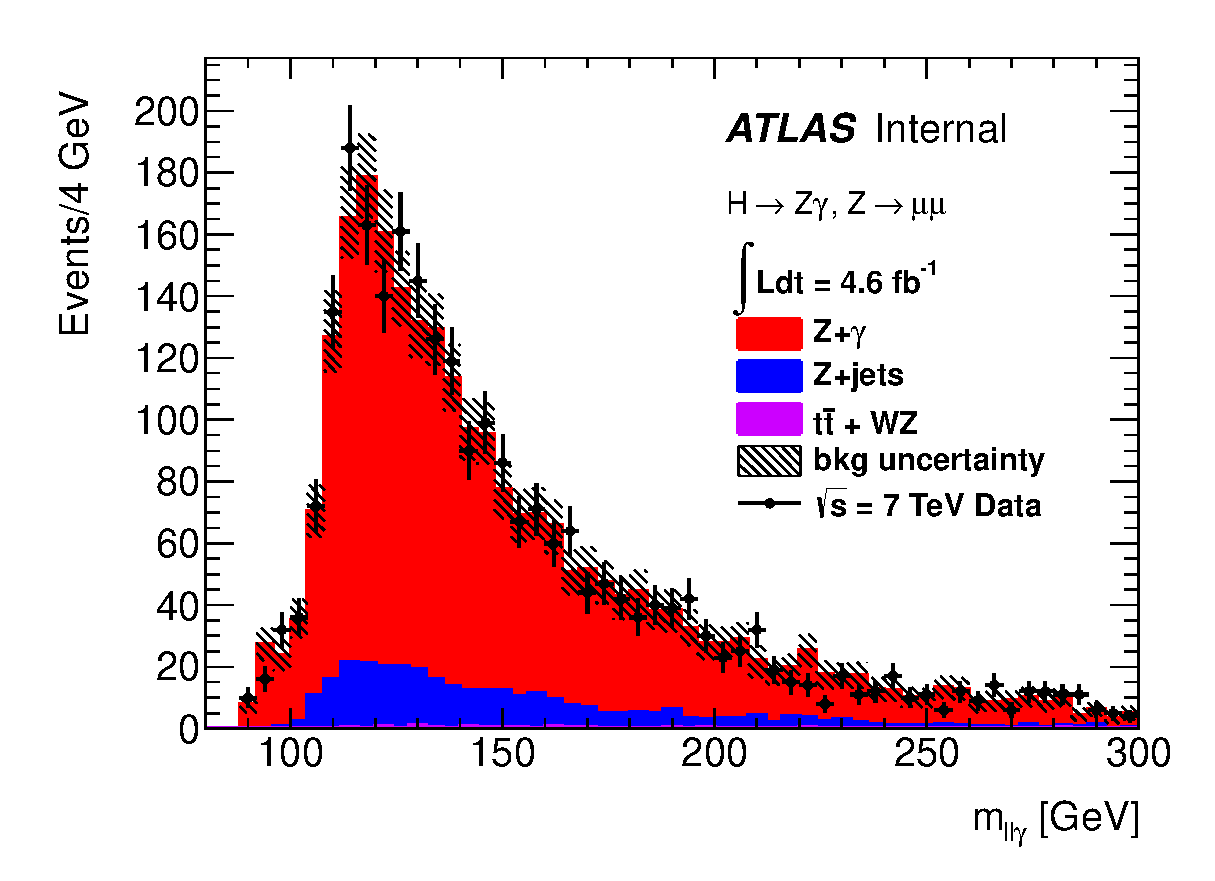
\includegraphics[width=0.49\columnwidth]{figures/bkg_decomposition_2011_mu_Mllg_Z_PV_corr_linscale}
    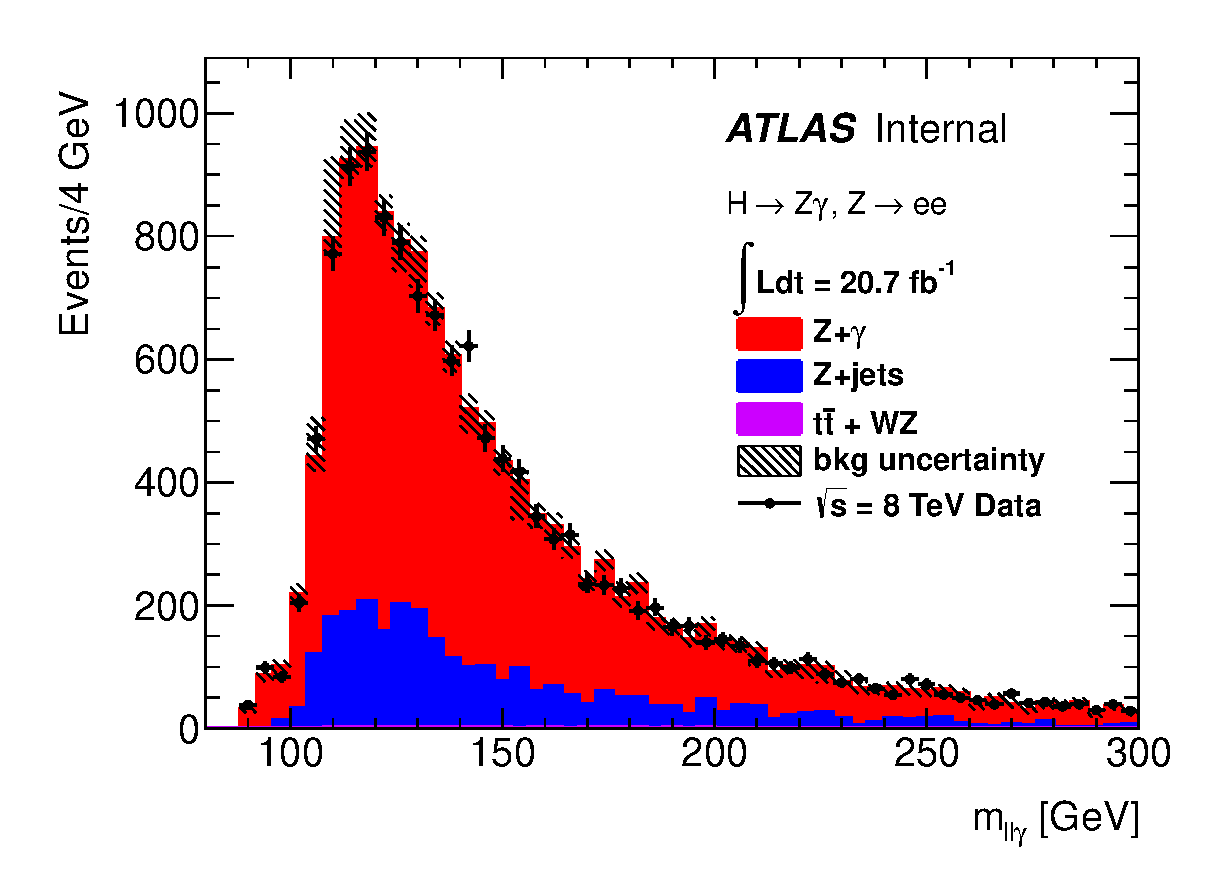
\includegraphics[width=0.49\columnwidth]{figures/bkg_decomposition_2012_e_Mllg_Z_PV_corr_linscale}
    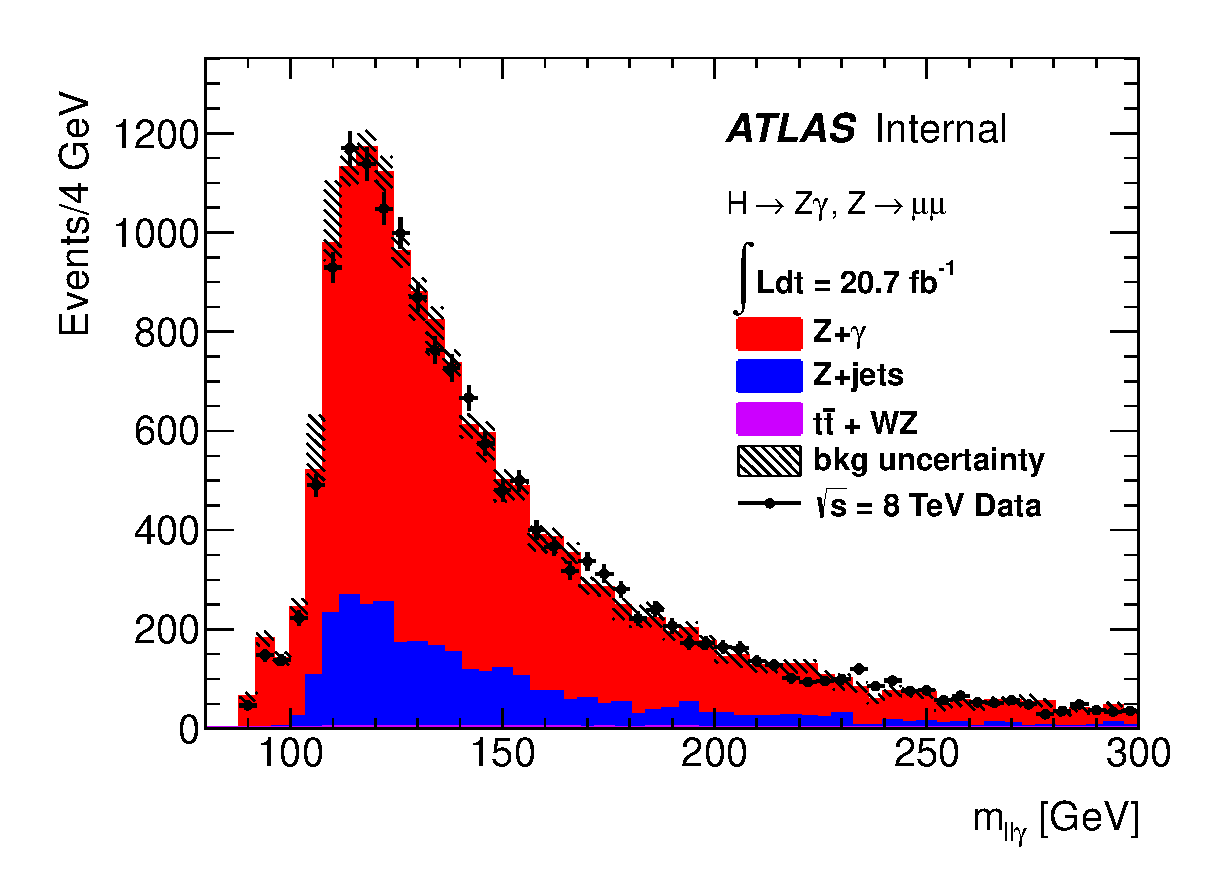
\includegraphics[width=0.49\columnwidth]{figures/bkg_decomposition_2012_mu_Mllg_Z_PV_corr_linscale}
    \caption{Three-body invariant mass $(m_{\ell\ell\gamma})$ distribution 
      of selected events in data (dots) and from the various
      background sources (histograms, from the simulation) normalized 
      to the yields determined as described in the text, 
      for $Z\to ee$ (left) and $Z\to\mu\mu$ (right) channels.
      The small peak near $m_Z$ is from residual FSR $Z$+$\gamma$ contamination.
      The background uncertainty includes statistical uncertainties and 
      systematic uncertainties from the inputs taken from the simulation, as detailed in the text.
    }
    \label{fig:zgamma_mass_linear}
  \end{center}
\end{figure}

\begin{figure}[!htbp]
  \begin{center}
    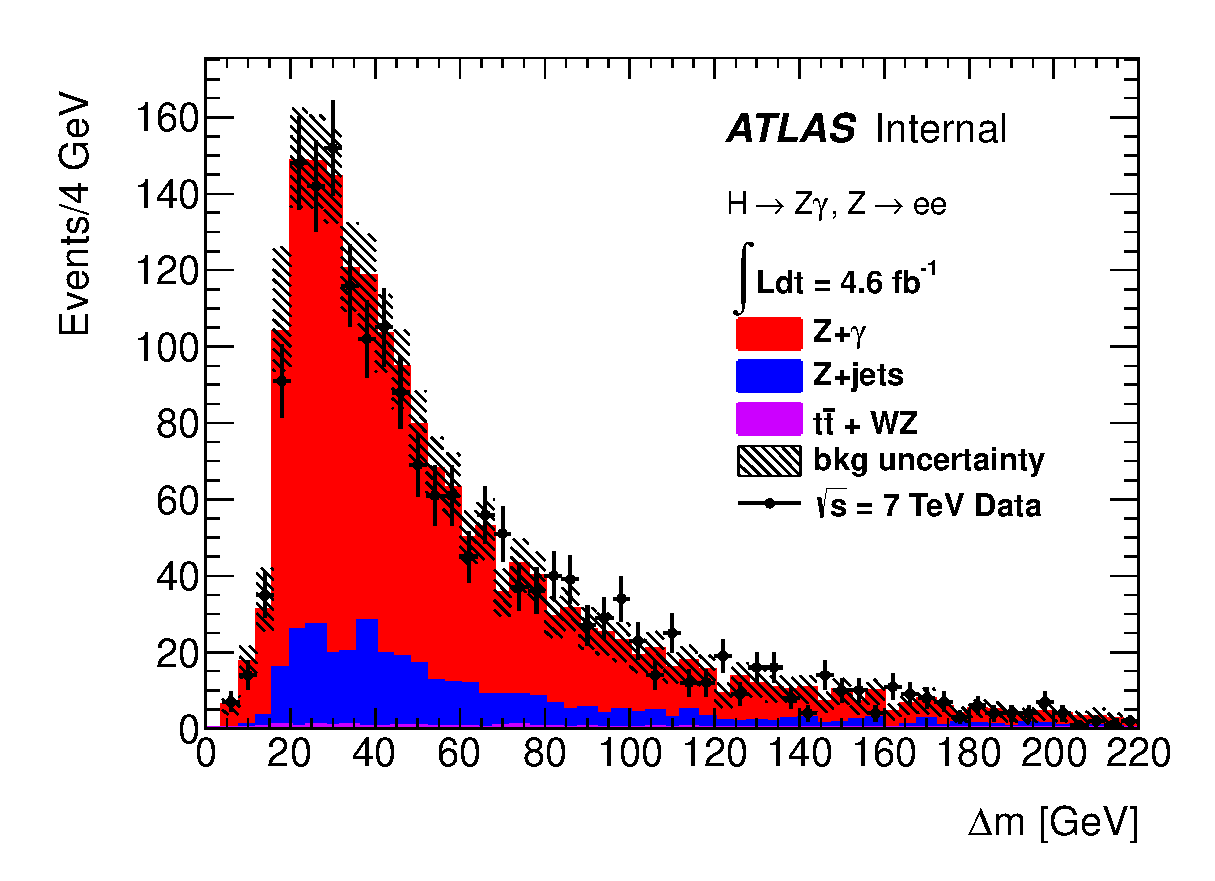
\includegraphics[width=0.49\columnwidth]{figures/bkg_decomposition_2011_e_dMllg_Z_PV_corr_linscale}
    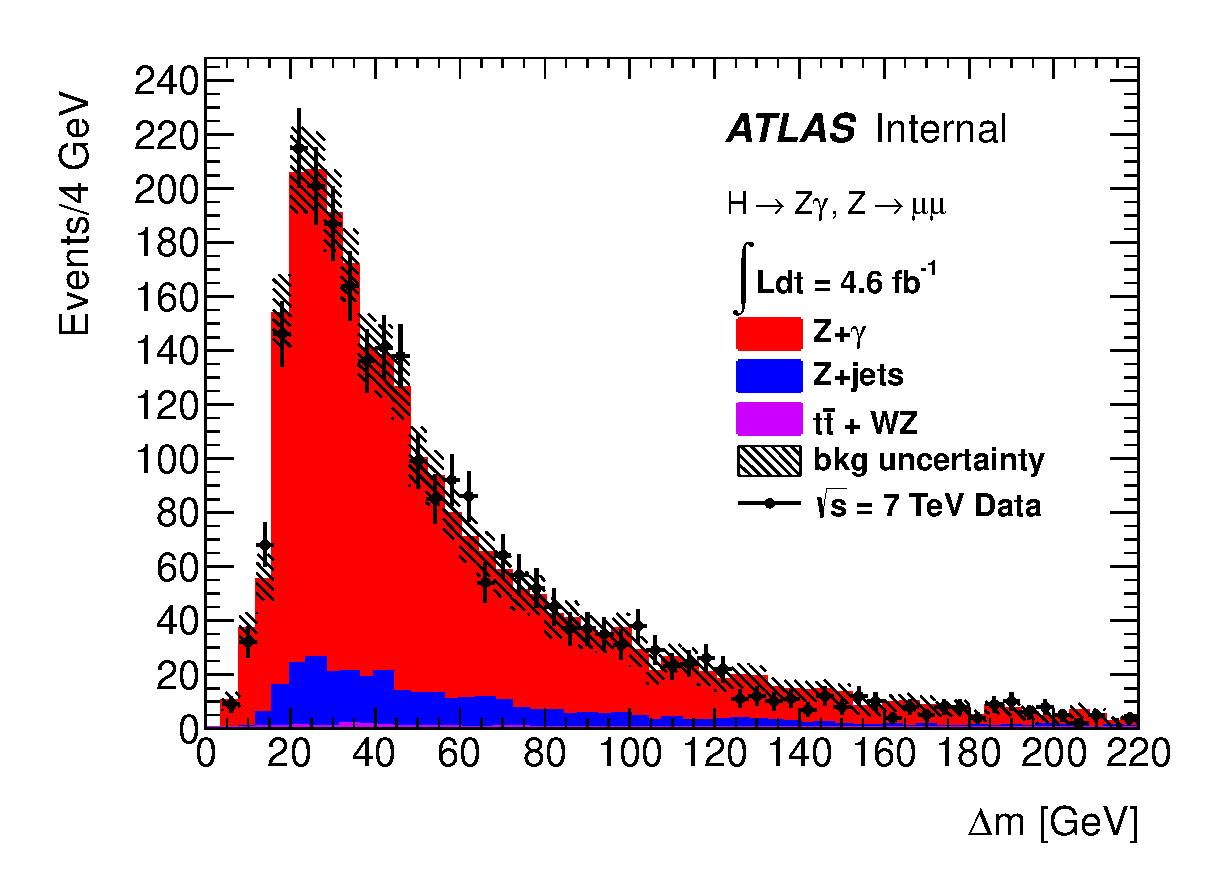
\includegraphics[width=0.49\columnwidth]{figures/bkg_decomposition_2011_mu_dMllg_Z_PV_corr_linscale}
    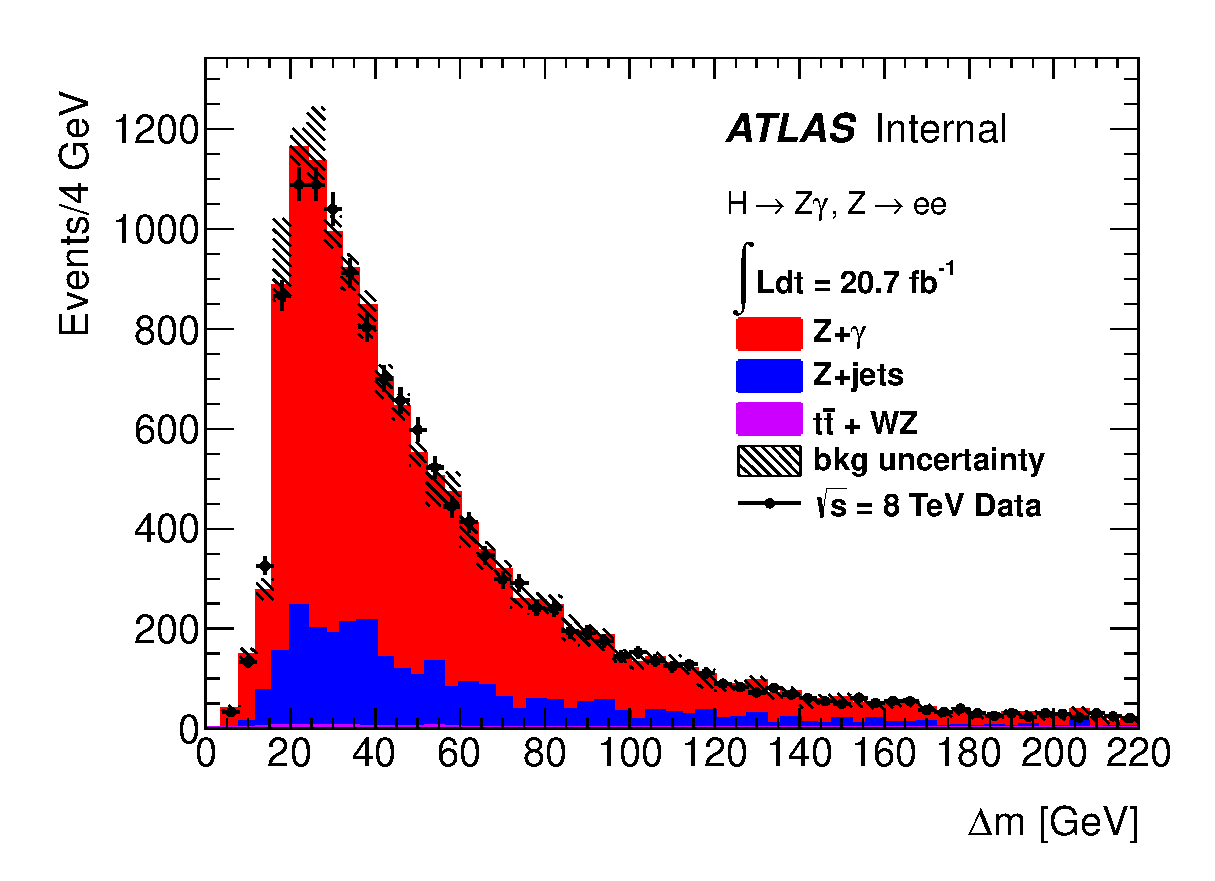
\includegraphics[width=0.49\columnwidth]{figures/bkg_decomposition_2012_e_dMllg_Z_PV_corr_linscale}
    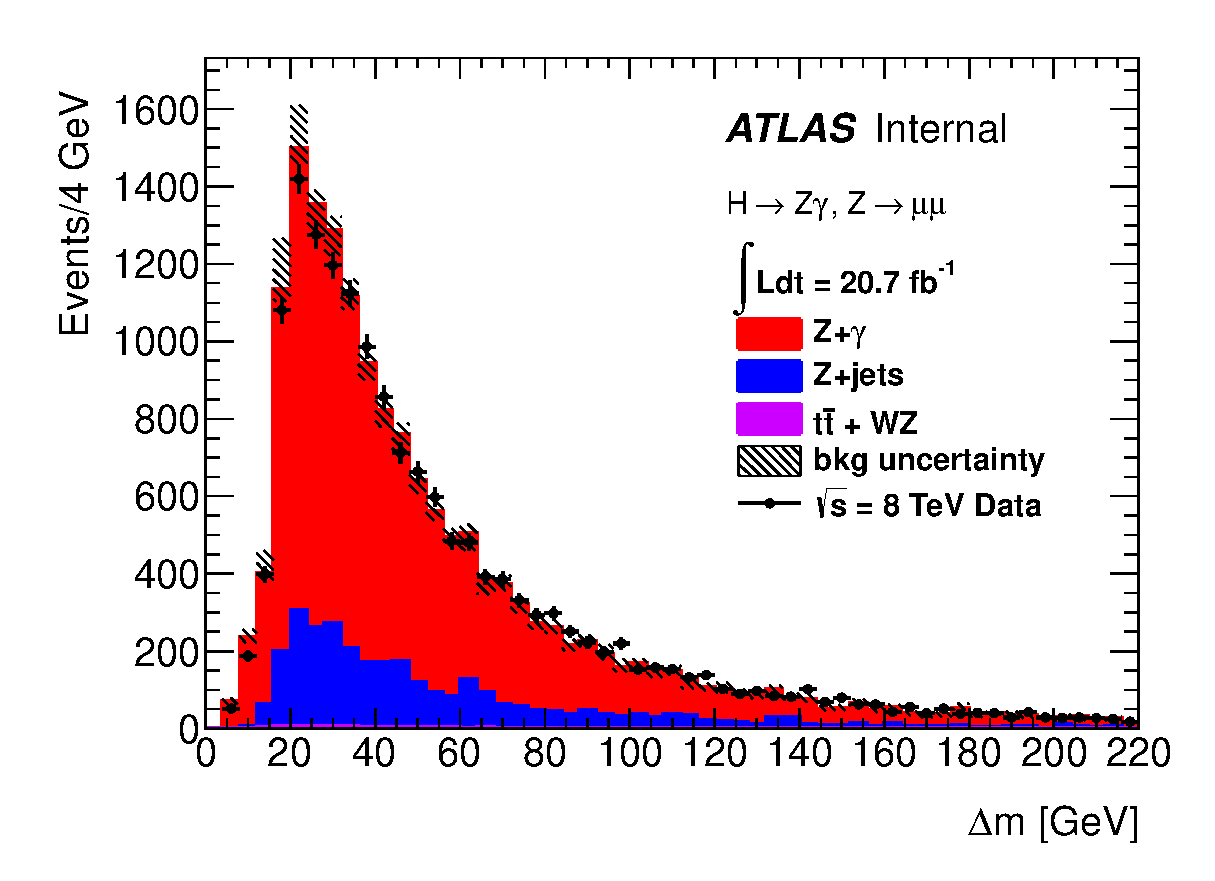
\includegraphics[width=0.49\columnwidth]{figures/bkg_decomposition_2012_mu_dMllg_Z_PV_corr_linscale}
    \caption{Distribution of the difference $\Delta m$ 
      between the final state three-body invariant mass
      $m_{\ell\ell\gamma}$ and the di-lepton invariant mass
      $m_{\ell\ell}$ for selected events in data (dots) and from
      the various background sources (histograms) normalized to the yields determined 
      as described in the text, for $Z\to ee$ (left) and $Z\to\mu\mu$ (right) channels.
      The background uncertainty includes statistical uncertainties and systematic
      uncertainties from the inputs taken from the simulation.
    }
    \label{fig:Dm_mass_linear}
  \end{center}
\end{figure}

\begin{figure}[!htbp]
  \begin{center}
  {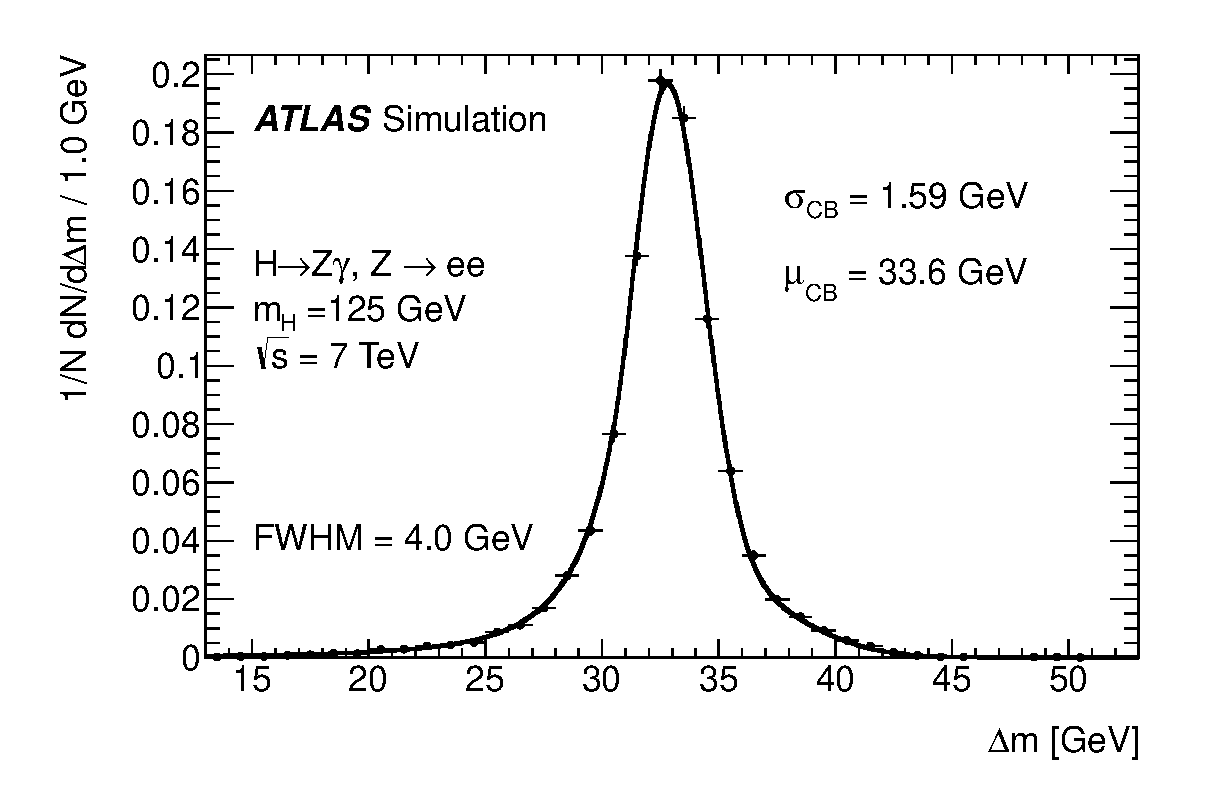
\includegraphics[width=0.46\textwidth]{figures/linPlot_125_EtaZgamma_Cat0_all_e_mc11c_mDif}}
  {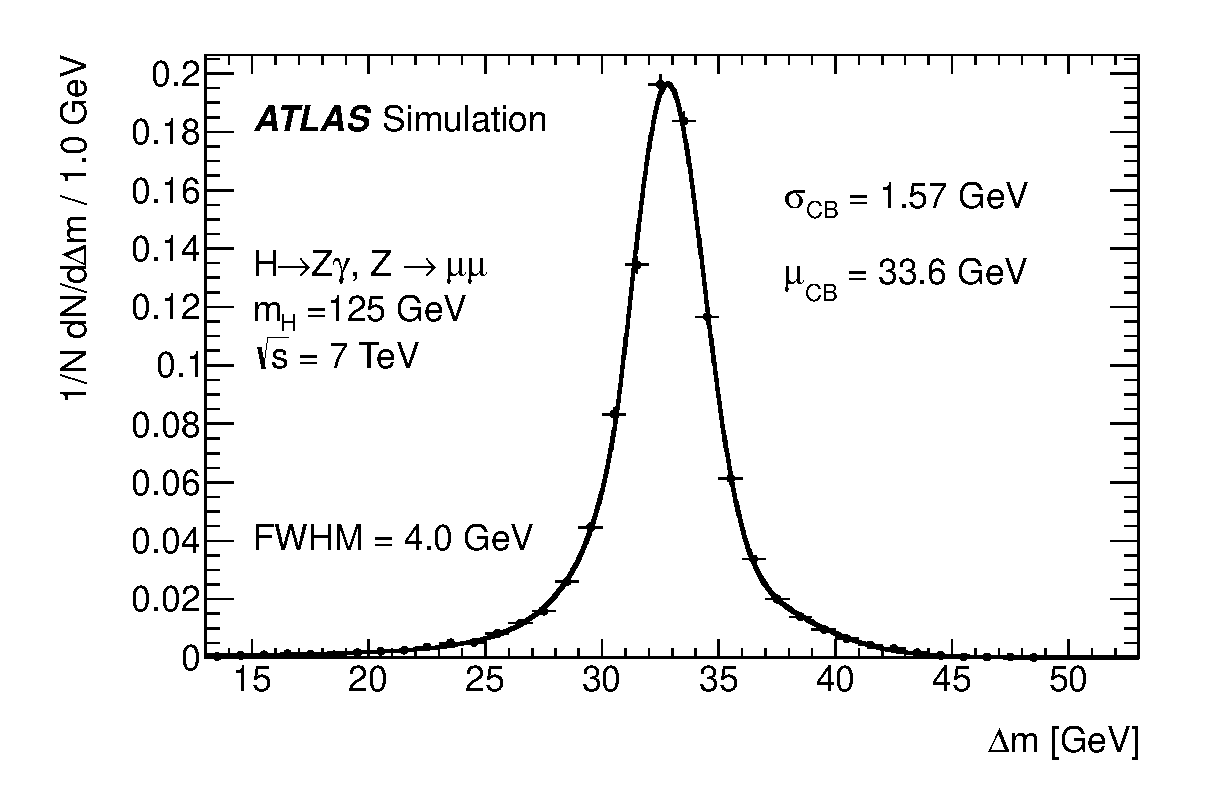
\includegraphics[width=0.46\textwidth]{figures/linPlot_125_EtaZgamma_Cat0_all_mu_mc11c_mDif}}
  {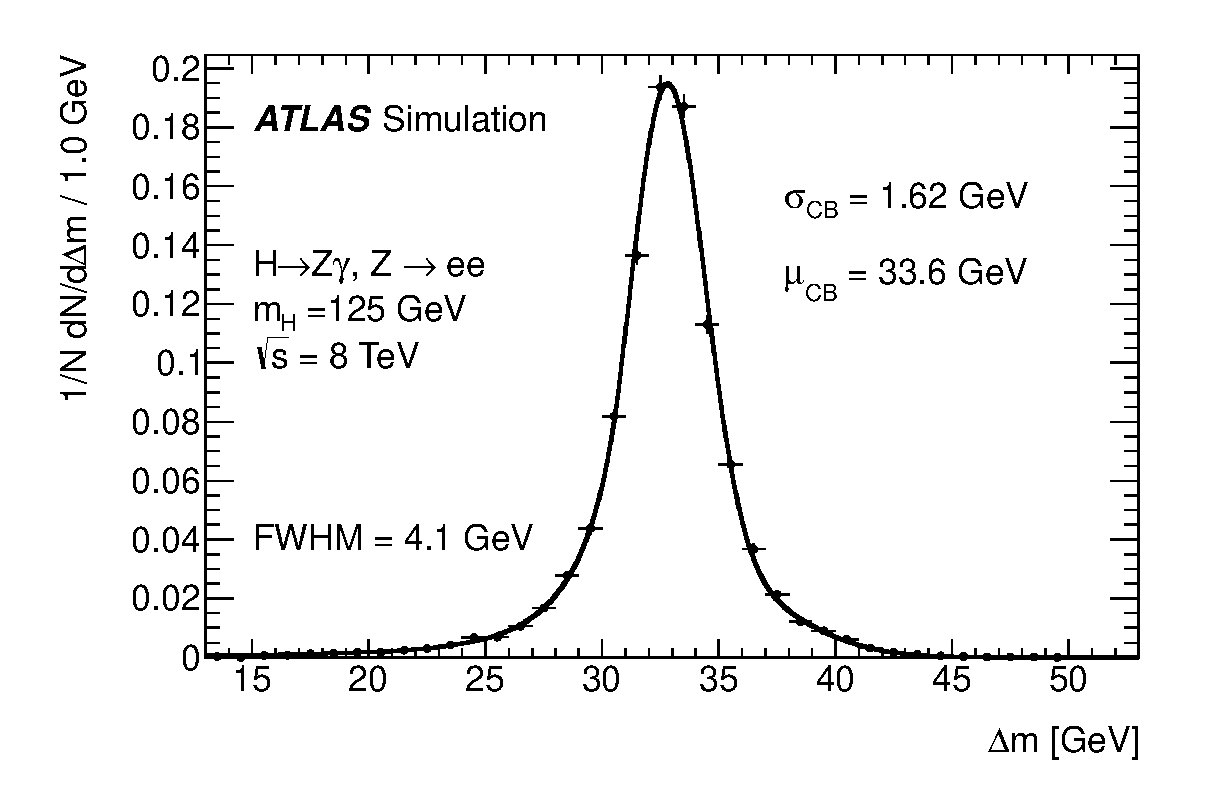
\includegraphics[width=0.46\textwidth]{figures/linPlot_125_EtaZgamma_Cat0_all_e_mc12a_mDif}}
  {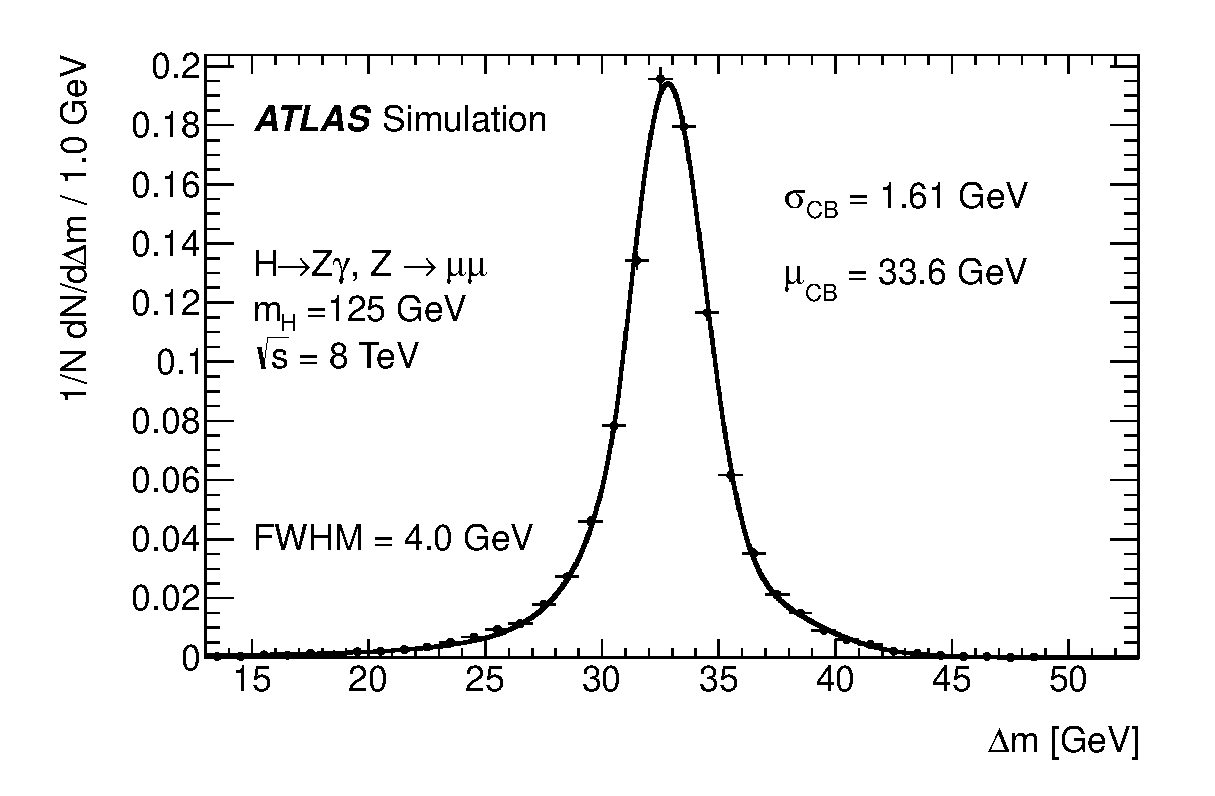
\includegraphics[width=0.46\textwidth]{figures/linPlot_125_EtaZgamma_Cat0_all_mu_mc12a_mDif}}
    \caption{Distribution (normalized to unit area) of the difference $\Delta m$ 
      between the final state three-body invariant mass
      $m_{\ell\ell\gamma}$ and the di-lepton invariant mass
      $m_{\ell\ell}$ for signal events
      passing the full selection (dots), for $m_H = 125$~GeV and $\sqrt{s}=7$ (top) or 8 (bottom) TeV. 
      The line overlaid represents the fit of the distribution with a
      model composed of the sum of a Crystal Ball (CB) and a Gaussian (GA) function.
      Left: electron channel, right: muon channel. 
    }
    \label{fig:resolution_model_example_8tev_H125}
  \end{center}
\end{figure}
 
 \begin{figure}[!htbp]
  \begin{center}
    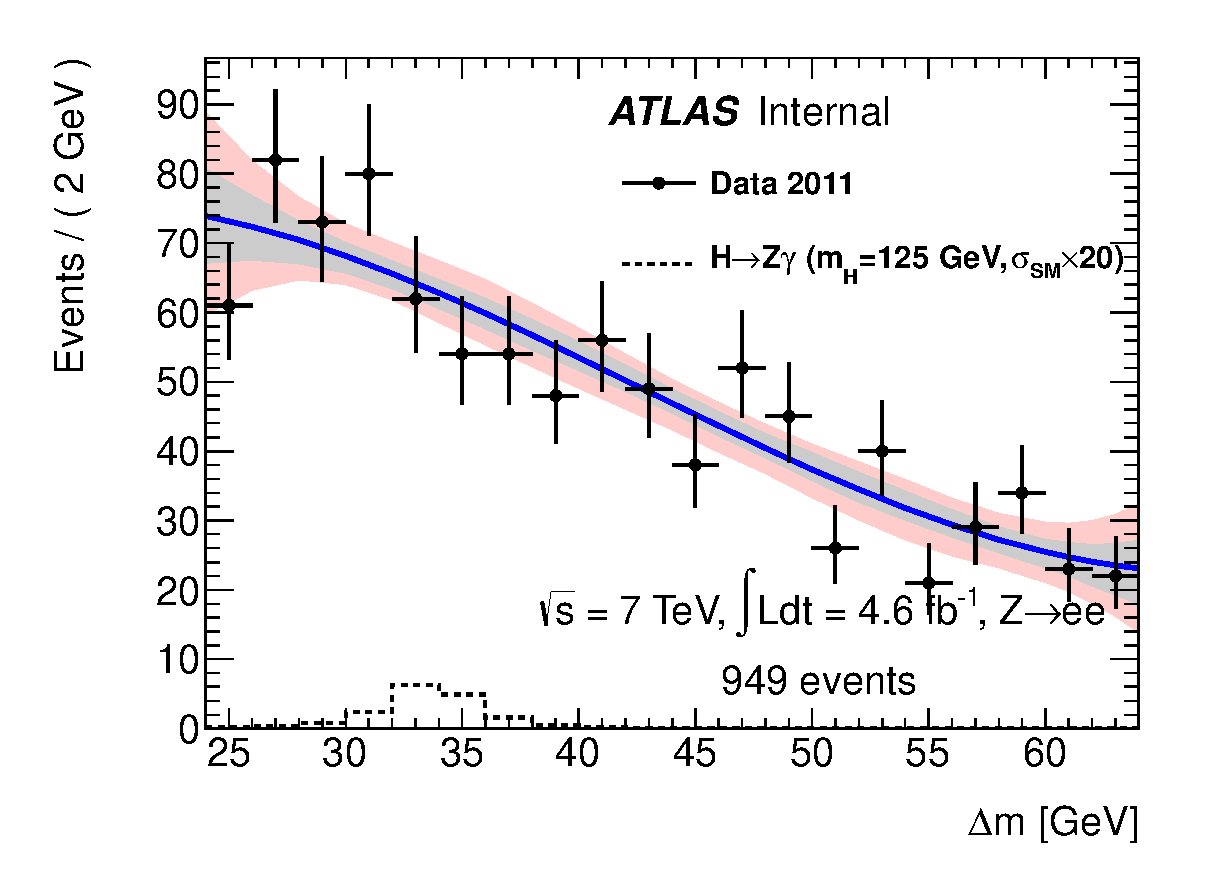
\includegraphics[width=0.49\columnwidth]{figures/bkgplots_e_deltaM_fit_11_CB3_fiterr_internal_withsignal}
    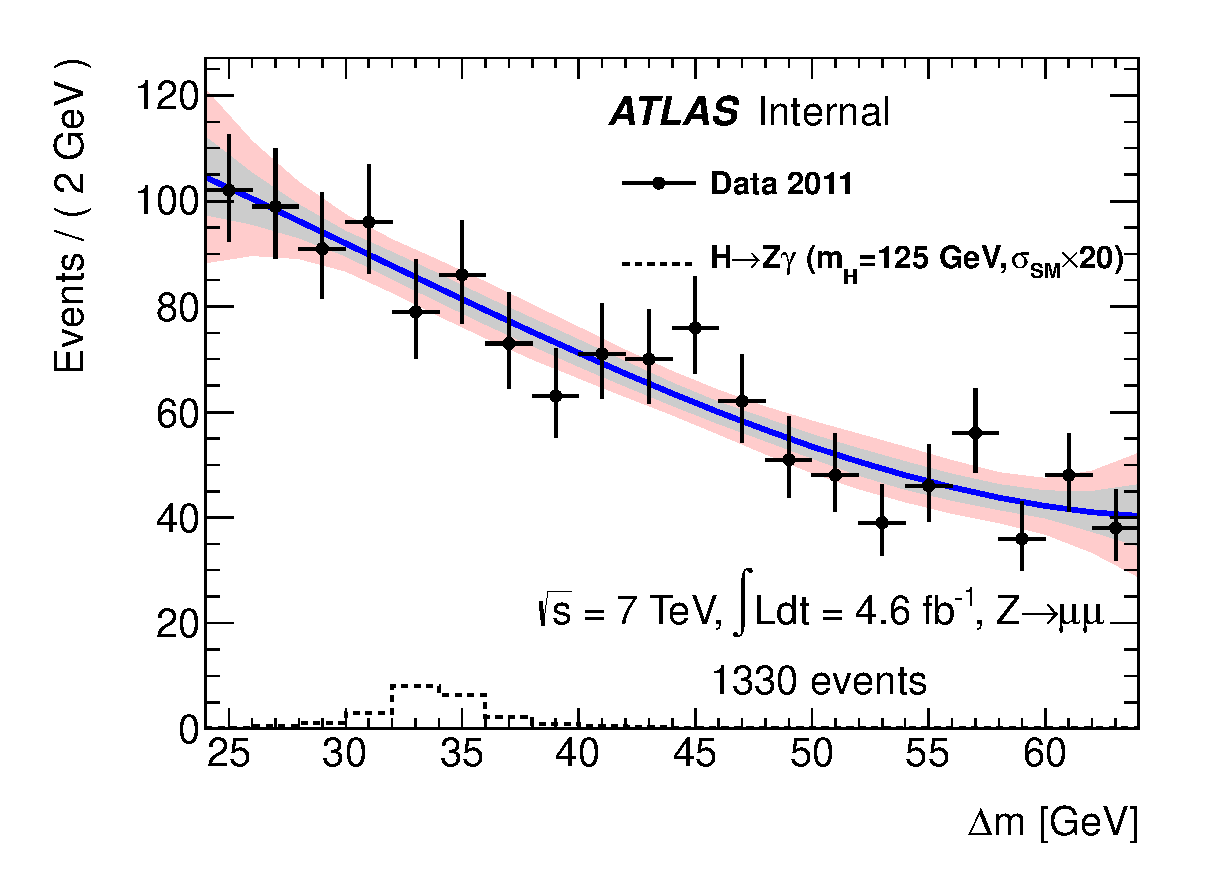
\includegraphics[width=0.49\columnwidth]{figures/bkgplots_mu_deltaM_fit_11_CB3_fiterr_internal_withsignal}
    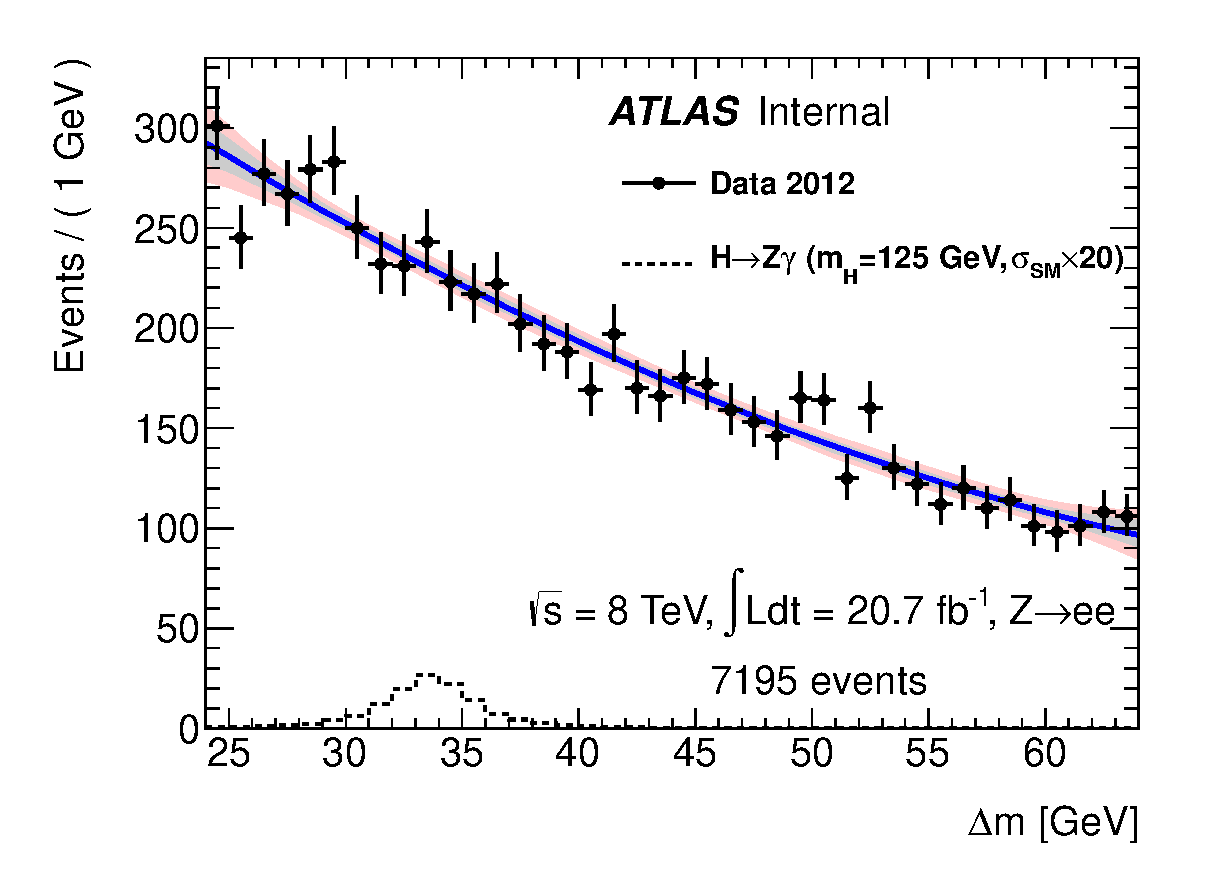
\includegraphics[width=0.49\columnwidth]{figures/bkgplots_e_deltaM_fit_12_CB3_fiterr_internal_withsignal} 
    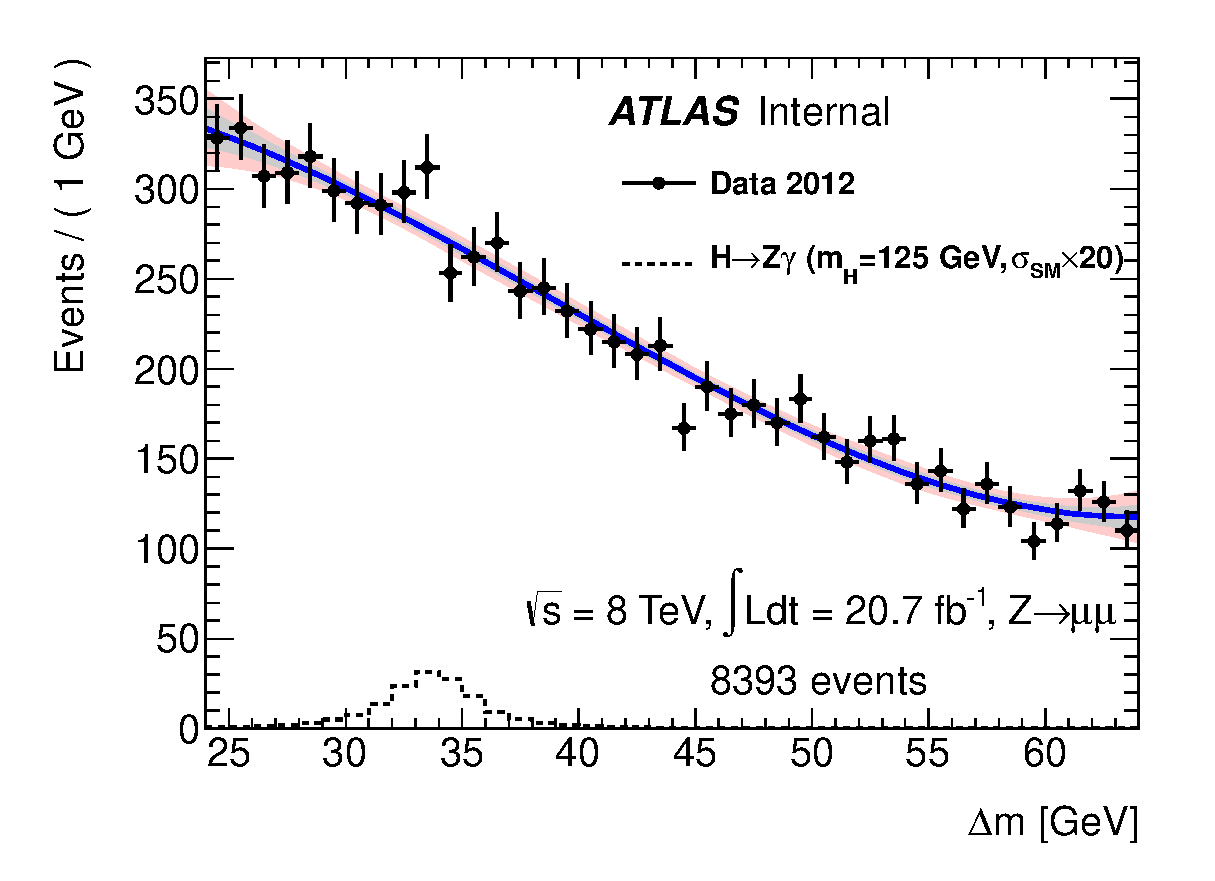
\includegraphics[width=0.49\columnwidth]{figures/bkgplots_mu_deltaM_fit_12_CB3_fiterr_internal_withsignal}
    \caption{Background-only fits to the distribution of 
      the mass difference $\Delta m$ of selected events in data,
      for $Z\to ee$ (left) and $Z\to\mu\mu$ (right), at $\sqrt{s}=7$ 
      TeV (top) or 8 TeV (bottom).
      For both 7 and 8 TeV, a third order polynomial is used for the fit.
      Dots correspond to data, the blue line is the fit result and the gray and light red
      bands are the 1$\sigma$ and 2$\sigma$ uncertainty 
      bands from the statistical uncertainties on the fitted 
      background model parameters.
      The dashed histograms correspond to the SM signal expectation,
      for a Higgs boson mass of 125 GeV, scaled by a factor 20 for clarity.
%%      The pulls of the data points with respect to the fit are also shown.
    }
    \label{fig:deltaM_data_bkgonly_fit}
  \end{center}
\end{figure}

\begin{figure}[!htbp]
\centering
    {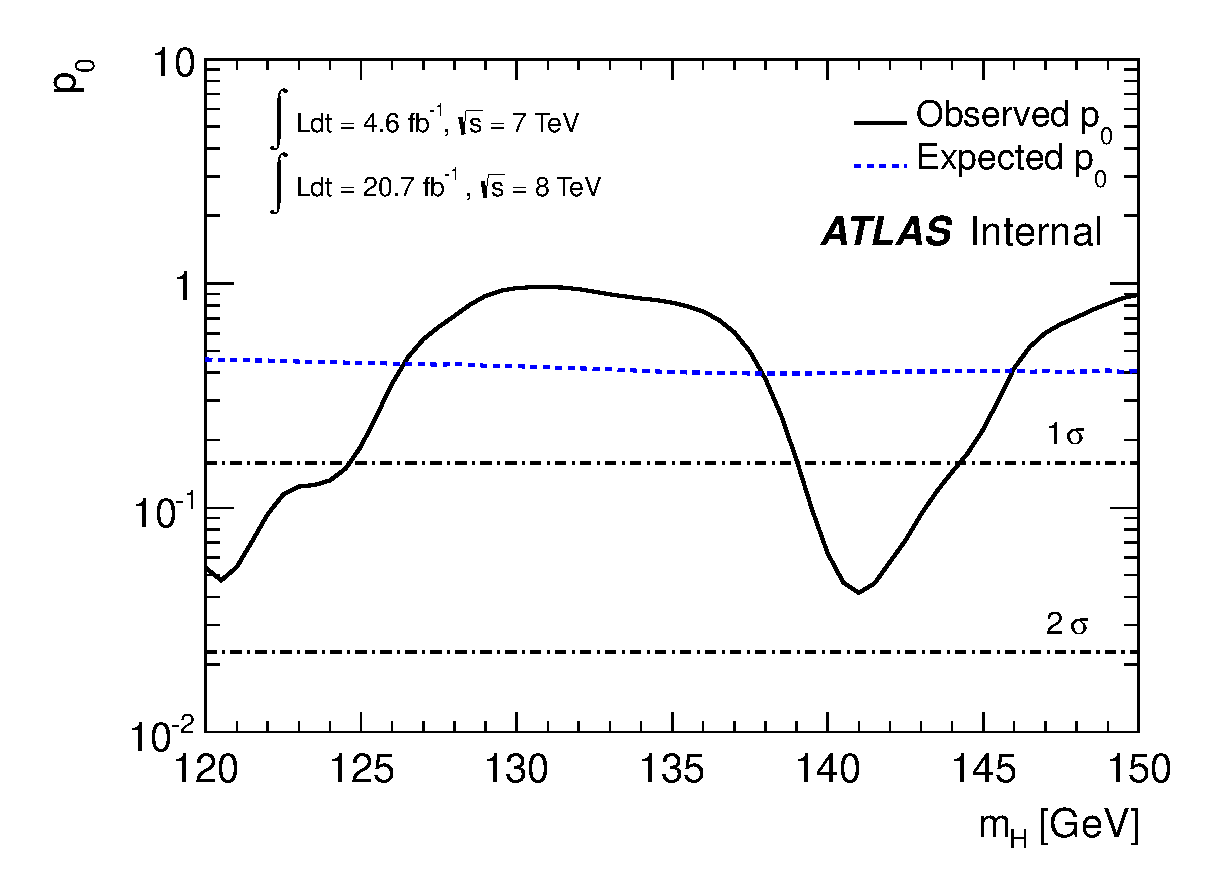
\includegraphics[totalheight=9cm,angle=0]{figures/plot_p0}}
    \caption{Expected (dashed blue line) and observed 
      (solid black line) $p_0$ (compatibility of
      the data with the background-only hypothesis) as a function
      of the Higgs boson mass, using \lumiseventev~\ifb\ of $pp$
      collisions at $\sqrt{s}=7$~TeV and \lumieighttev~\ifb\ of $pp$
      collisions at $\sqrt{s}=8$~TeV.}
    \label{fig:ExpectedP0_1}
\end{figure}

\begin{figure}[!htbp]
\centering
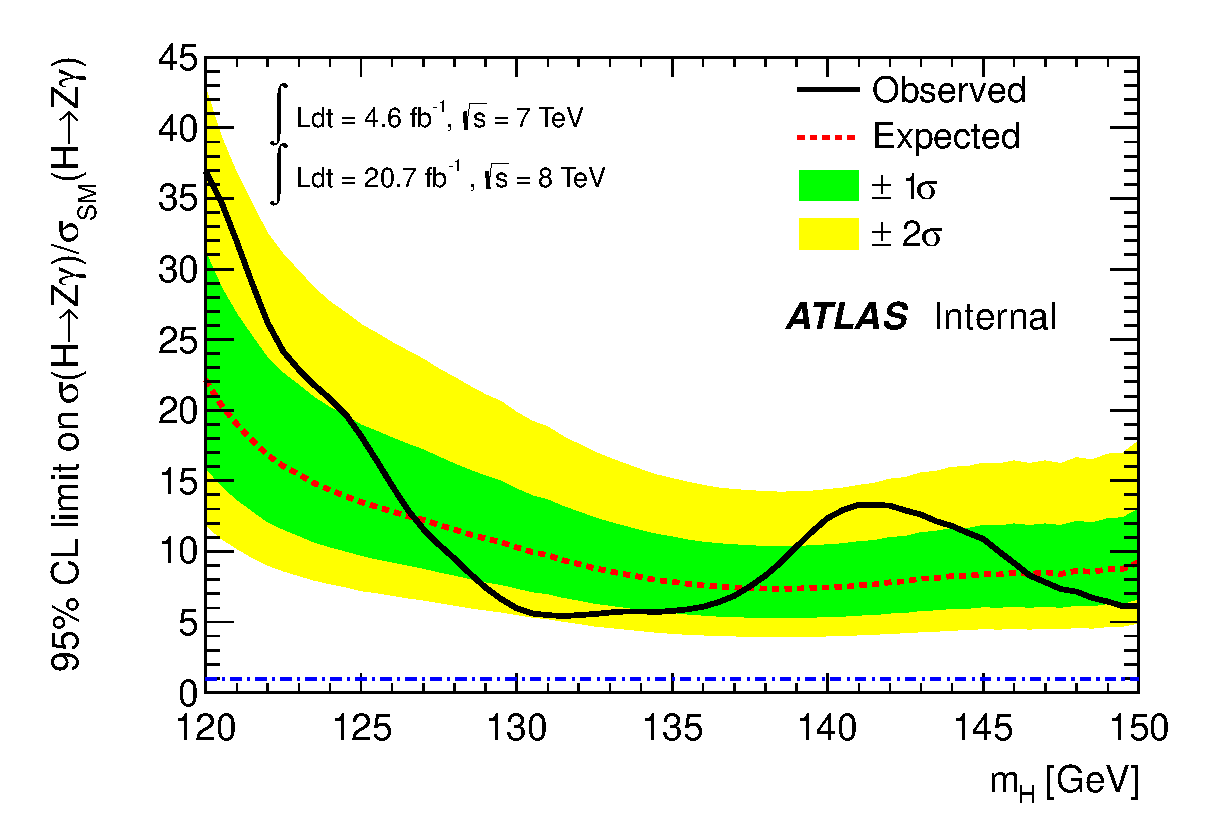
\includegraphics[totalheight=9cm,angle=0]{figures/plot_smooth_cls}
\caption{Observed 95\% $CL$ limits (solid black line) 
  on the production cross section of a SM Higgs boson 
  decaying to $Z\gamma$, as a function of the Higgs boson 
  mass, using \lumiseventev~\ifb\ of $pp$
  collisions at $\sqrt{s}=7$~TeV and \lumieighttev~\ifb\ of $pp$
  collisions at $\sqrt{s}=8$~TeV.
  The median expected 95\% $CL$ exclusion limits (dashed red line)
  are also shown. The green and yellow bands correspond to the $\pm 1\sigma$ 
  and $\pm2\sigma$ intervals.
}
\label{fig:ExpectedExclusion_1}
\end{figure}
